\documentclass[11pt]{article}

\usepackage[utf8]{inputenc}
\usepackage[a4paper,margin=0.85in]{geometry}
\usepackage{amsmath,amssymb}
\usepackage{enumitem}
\usepackage{parskip}
\usepackage{xcolor}
\usepackage{fancyhdr}
\usepackage{tikz}
\usepackage{graphicx}
\usepackage{eso-pic}
\usepackage{titlesec}
\usepackage{listings}
\usepackage{hyperref}

\graphicspath{{../}{./}}
\definecolor{kcpc-text}{RGB}{20,20,20}
\definecolor{kcpc-muted}{RGB}{90,90,90}
\definecolor{kcpc-red}{RGB}{176,0,0}

\pagestyle{fancy}
\fancyhf{}
\lhead{\textcolor{kcpc-text}{\small\bfseries Solutions}}
\rhead{\textcolor{kcpc-muted}{\small Week 5}}
\cfoot{\textcolor{kcpc-muted}{\small KCPC \quad\thepage}}
\renewcommand{\headrulewidth}{0.4pt}
\renewcommand{\headrule}{\hbox to\headwidth{\color{kcpc-red}\leaders\hrule height \headrulewidth\hfill}}
\setlength{\headheight}{28pt}

\AddToShipoutPictureBG{%
  \begin{tikzpicture}[remember picture,overlay]
    \node[opacity=0.035,at=(current page.center)]{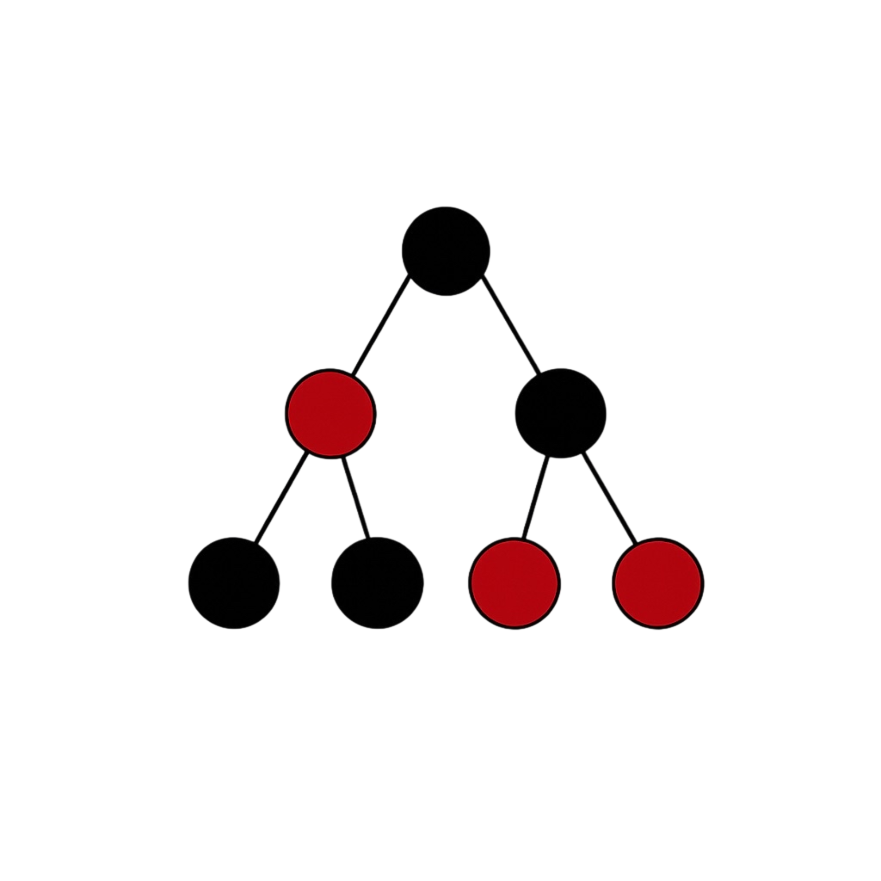
\includegraphics[width=0.38\paperwidth]{kcpc-logo.png}};
  \end{tikzpicture}%
}

\titleformat{\section}{\large\bfseries\color{kcpc-red}}{\thesection}{1em}{}
\newcommand{\insight}[1]{\par\medskip\noindent\textbf{Key idea:} #1}
\newcommand{\correct}[1]{\par\textbf{Correctness:} #1}
\newcommand{\bounds}[1]{\par\textbf{Time and space:} #1}
\newcommand{\pitfalls}[1]{\par\textbf{Pitfalls:} #1}

\lstset{
  basicstyle=\ttfamily\footnotesize,
  breaklines=true,
  columns=fullflexible,
  keepspaces=true,
  frame=single,
  showstringspaces=false,
  captionpos=t,
}

\hypersetup{colorlinks=true,urlcolor=kcpc-red,linkcolor=kcpc-red}
\setlength{\emergencystretch}{2em}

\title{KCPC Week 5 Solutions\\Graphs II: Dijkstra and 0--1 BFS}
\author{}
\date{}

\begin{document}
\maketitle\thispagestyle{fancy}

These solutions accompany problems on the Workshop 5 problem sheet. Problems 1--11 have both Python 3 and C++17 implementations, but homework problems 12--15 only have C++17 implementations.

\section*{I. Integrated examples}

\section{GeeksForGeeks --- Dijkstra Algorithm}
\href{https://www.geeksforgeeks.org/problems/implementing-dijkstra-set-1-adjacency-matrix/1}{Original problem / current judge page}

Despite ``Adjacency Matrix'' in the URL, the judge takes an \textbf{edge list}: \texttt{dijkstra(V, edges, src)}, with each row \texttt{[u,v,w]}. The graph is undirected and connected, and weights are non-negative. The statement guarantees that shortest distances fit in a signed 32-bit integer.
\insight{Build both adjacency directions, then run min-heap Dijkstra from \texttt{src}.}
\correct{Start with distance zero at the source. Each relaxation extends a known path by one edge. Since weights are non-negative, the Dijkstra argument in the problem sheet's \emph{A quick reminder} shows that each finalised distance is shortest. The graph is connected, so every vertex is reached.}
\bounds{For $V$ vertices and $E$ undirected edges: $O(V+E\log(E+2))$ time and $O(V+E)$ total auxiliary space, including the adjacency list and an $O(E+1)$ lazy heap.}
\pitfalls{\texttt{edges} is an edge list, not a list of neighbours for each vertex. Add both directions, and remember that weights can be zero. The C++ code uses 64-bit sums, then converts to \texttt{vector<int>} because the judge guarantees the answers fit.}

% LISTING p01-python: GeeksForGeeks judge class
\begin{lstlisting}[language=Python,caption={P01 --- Python 3},label={lst:p01-python}]
from heapq import heappop, heappush

class Solution:
    def dijkstra(self, V: int, edges: list[list[int]],
                 src: int) -> list[int]:
        adj = [[] for _ in range(V)]
        for u, v, w in edges:
            adj[u].append((v, w))
            adj[v].append((u, w))
        dist = [float('inf')] * V
        dist[src] = 0
        heap = [(0, src)]
        while heap:
            d, u = heappop(heap)
            if d != dist[u]:
                continue
            for v, w in adj[u]:
                nd = d + w
                if nd < dist[v]:
                    dist[v] = nd
                    heappush(heap, (nd, v))
        return dist
\end{lstlisting}
% LISTING p01-cpp: GeeksForGeeks judge class
\begin{lstlisting}[language=C++,caption={P01 --- C++17},label={lst:p01-cpp}]
#include <functional>
#include <queue>
#include <utility>
#include <vector>
using namespace std;
class Solution {
public:
    vector<int> dijkstra(int V, vector<vector<int>>& edges,
                         int src) {
        using ll = long long;
        const ll INF = (1LL << 62);
        vector<vector<pair<int, int>>> adj(V);
        for (const auto& e : edges) {
            adj[e[0]].push_back({e[1], e[2]});
            adj[e[1]].push_back({e[0], e[2]});
        }
        vector<ll> dist(V, INF);
        using State = pair<ll, int>;
        priority_queue<State, vector<State>, greater<State>> pq;
        dist[src] = 0;
        pq.push({0, src});
        while (!pq.empty()) {
            auto [d, u] = pq.top(); pq.pop();
            if (d != dist[u]) continue;
            for (auto [v, w] : adj[u]) {
                if (d + w < dist[v]) {
                    dist[v] = d + w;
                    pq.push({dist[v], v});
                }
            }
        }
        return vector<int>(dist.begin(), dist.end());
    }
};
\end{lstlisting}

\section{LeetCode 743 --- Network Delay Time}
\href{https://leetcode.com/problems/network-delay-time/}{Problem statement}
\insight{Run Dijkstra from $k$ to find when each vertex first receives the signal. The answer is the largest of these arrival times.}
\correct{The time taken along a directed path is the sum of its edge weights, so Dijkstra finds the earliest arrival at each vertex. We need to wait until the last vertex receives the signal. If any vertex is unreachable, the signal can never reach the whole network.}
\bounds{With $n$ vertices and $m$ directed edges, $O(n+m\log(m+2))$ time and $O(n+m)$ space, including an $O(m+1)$ heap.}
\pitfalls{Edges are directed. Labels are 1-based; index zero is not a vertex. Take the maximum, not the sum, and return $-1$ for an unreachable vertex.}
% LISTING p02-python: LeetCode judge class
\begin{lstlisting}[language=Python,caption={P02 --- Python 3},label={lst:p02-python}]
from heapq import heappop, heappush
from typing import List

class Solution:
    def networkDelayTime(self, times: List[List[int]],
                         n: int, k: int) -> int:
        adj = [[] for _ in range(n + 1)]
        for u, v, w in times:
            adj[u].append((v, w))
        dist = [float('inf')] * (n + 1)
        dist[k] = 0
        heap = [(0, k)]
        while heap:
            d, u = heappop(heap)
            if d != dist[u]:
                continue
            for v, w in adj[u]:
                if d + w < dist[v]:
                    dist[v] = d + w
                    heappush(heap, (dist[v], v))
        answer = max(dist[1:])
        return -1 if answer == float('inf') else answer
\end{lstlisting}
% LISTING p02-cpp: LeetCode judge class
\begin{lstlisting}[language=C++,caption={P02 --- C++17},label={lst:p02-cpp}]
#include <algorithm>
#include <functional>
#include <queue>
#include <utility>
#include <vector>
using namespace std;
class Solution {
public:
    int networkDelayTime(vector<vector<int>>& times, int n, int k) {
        const int INF = 1000000000;
        vector<vector<pair<int, int>>> adj(n + 1);
        for (const auto& e : times)
            adj[e[0]].push_back({e[1], e[2]});
        vector<int> dist(n + 1, INF);
        using State = pair<int, int>;
        priority_queue<State, vector<State>, greater<State>> pq;
        dist[k] = 0;
        pq.push({0, k});
        while (!pq.empty()) {
            auto [d, u] = pq.top(); pq.pop();
            if (d != dist[u]) continue;
            for (auto [v, w] : adj[u]) {
                if (d + w < dist[v]) {
                    dist[v] = d + w;
                    pq.push({dist[v], v});
                }
            }
        }
        int ans = *max_element(dist.begin() + 1, dist.end());
        return ans == INF ? -1 : ans;
    }
};
\end{lstlisting}

\section{LeetCode 1368 --- Minimum Cost to Make at Least One Valid Path in a Grid}
\href{https://leetcode.com/problems/minimum-cost-to-make-at-least-one-valid-path-in-a-grid/}{Problem statement}
\insight{An edge \emph{leaving} a cell costs zero if it follows that cell's arrow, otherwise one. Use 0--1 BFS. Arrow codes are $1=$right, $2=$left, $3=$down, $4=$up.}
\correct{Take a path that doesn't revisit any cell. Changing each arrow that points the wrong way makes this path valid, and its graph cost counts exactly those changes. We can always remove cycles without increasing the cost, so revisiting cells cannot give a better answer. In the other direction, a valid path through a modified grid uses no more changed arrows than the total number of changes. The minimum path cost is therefore the minimum number of changes, which 0--1 BFS finds.}
\bounds{For $R C$ cells there are at most $4RC$ edges: $O(RC)$ time and $O(RC)$ space for distances and the deque.}
\pitfalls{Check the arrow in the cell you're leaving, not the one you're entering. Don't mark a cell as finished when it first enters the deque: a later zero-cost route may improve its distance. If an arrow points outside the grid, there is no free move in that direction.}
% LISTING p03-python: LeetCode judge class
\begin{lstlisting}[language=Python,caption={P03 --- Python 3},label={lst:p03-python}]
from collections import deque
from typing import List

class Solution:
    def minCost(self, grid: List[List[int]]) -> int:
        rows, cols = len(grid), len(grid[0])
        moves = [(0, 1), (0, -1), (1, 0), (-1, 0)]
        dist = [[float('inf')] * cols for _ in range(rows)]
        dist[0][0] = 0
        queue = deque([(0, 0, 0)])
        while queue:
            d, r, c = queue.popleft()
            if d != dist[r][c]:
                continue
            for code, (dr, dc) in enumerate(moves, 1):
                nr, nc = r + dr, c + dc
                if 0 <= nr < rows and 0 <= nc < cols:
                    w = int(grid[r][c] != code)
                    if d + w < dist[nr][nc]:
                        dist[nr][nc] = d + w
                        item = (d + w, nr, nc)
                        if w:
                            queue.append(item)
                        else:
                            queue.appendleft(item)
        return dist[-1][-1]
\end{lstlisting}
% LISTING p03-cpp: LeetCode judge class
\begin{lstlisting}[language=C++,caption={P03 --- C++17},label={lst:p03-cpp}]
#include <array>
#include <deque>
#include <vector>
using namespace std;
class Solution {
public:
    int minCost(vector<vector<int>>& grid) {
        int R = grid.size(), C = grid[0].size();
        int dr[] = {0, 0, 1, -1}, dc[] = {1, -1, 0, 0};
        vector<vector<int>> dist(R, vector<int>(C, 1000000000));
        deque<array<int, 3>> dq;
        dist[0][0] = 0;
        dq.push_back({0, 0, 0});
        while (!dq.empty()) {
            auto [d, r, c] = dq.front(); dq.pop_front();
            if (d != dist[r][c]) continue;
            for (int k = 0; k < 4; ++k) {
                int nr = r + dr[k], nc = c + dc[k];
                if (nr < 0 || nr >= R || nc < 0 || nc >= C) continue;
                int w = (grid[r][c] != k + 1);
                if (d + w < dist[nr][nc]) {
                    dist[nr][nc] = d + w;
                    if (w) dq.push_back({d + w, nr, nc});
                    else dq.push_front({d, nr, nc});
                }
            }
        }
        return dist[R - 1][C - 1];
    }
};
\end{lstlisting}

\section*{II. Core practice}

\section{LeetCode 1514 --- Path with Maximum Probability}
\href{https://leetcode.com/problems/path-with-maximum-probability/}{Problem statement}
\insight{Store the best probability found for each vertex, and use a max-heap to try the most likely path first. Multiply by the edge probability when extending a path.}
\correct{Every edge probability lies in $[0,1]$, so adding an edge cannot make a path more likely. Dijkstra's argument still works, but with products and a max-heap instead of sums and a min-heap. When we pop a vertex with its current best probability, that probability is optimal. We can stop as soon as this happens for the destination.}
\bounds{For $n$ vertices and $m$ undirected edges: $O(n+m\log(m+2))$ time and $O(n+m)$ space; lazy heap space is $O(m+1)$.}
\pitfalls{The graph is undirected; multiply probabilities, do not add them. Python negates heap keys. Use \texttt{double} in C++, and compare with a tolerance only in tests, not in relaxation logic. An unreachable destination has answer zero; the empty start-to-start path has probability one.}
% LISTING p04-python: LeetCode judge class
\begin{lstlisting}[language=Python,caption={P04 --- Python 3},label={lst:p04-python}]
from heapq import heappop, heappush
from typing import List

class Solution:
    def maxProbability(self, n: int, edges: List[List[int]],
                       succProb: List[float], start_node: int,
                       end_node: int) -> float:
        adj = [[] for _ in range(n)]
        for (u, v), p in zip(edges, succProb):
            adj[u].append((v, p))
            adj[v].append((u, p))
        best = [0.0] * n
        best[start_node] = 1.0
        heap = [(-1.0, start_node)]
        while heap:
            negp, u = heappop(heap)
            p = -negp
            if p < best[u]:
                continue
            if u == end_node:
                return p
            for v, probability in adj[u]:
                candidate = p * probability
                if candidate > best[v]:
                    best[v] = candidate
                    heappush(heap, (-candidate, v))
        return 0.0
\end{lstlisting}
% LISTING p04-cpp: LeetCode judge class
\begin{lstlisting}[language=C++,caption={P04 --- C++17},label={lst:p04-cpp}]
#include <queue>
#include <utility>
#include <vector>
using namespace std;
class Solution {
public:
    double maxProbability(int n, vector<vector<int>>& edges,
                          vector<double>& succProb, int start_node,
                          int end_node) {
        vector<vector<pair<int, double>>> adj(n);
        for (int i = 0; i < (int)edges.size(); ++i) {
            int u = edges[i][0], v = edges[i][1];
            adj[u].push_back({v, succProb[i]});
            adj[v].push_back({u, succProb[i]});
        }
        vector<double> best(n, 0.0);
        priority_queue<pair<double, int>> pq;
        best[start_node] = 1.0;
        pq.push({1.0, start_node});
        while (!pq.empty()) {
            auto [p, u] = pq.top(); pq.pop();
            if (p < best[u]) continue;
            if (u == end_node) return p;
            for (auto [v, probability] : adj[u]) {
                double candidate = p * probability;
                if (candidate > best[v]) {
                    best[v] = candidate;
                    pq.push({candidate, v});
                }
            }
        }
        return 0.0;
    }
};
\end{lstlisting}

\section{LeetCode 1631 --- Path with Minimum Effort}
\href{https://leetcode.com/problems/path-with-minimum-effort/}{Problem statement}
\insight{A path's effort is its largest edge difference. Replace additive relaxation by $\max(d[u], |h[u]-h[v]|)$.}
\correct{Each stored effort comes from a path we've found. Extending that path cannot lower its largest height difference, and a smaller effort at a cell can never give a worse result when taking the same next step. Dijkstra's argument therefore works with maximum in place of addition. When the destination is finalised, its effort is the smallest possible.}
\bounds{With $N=RC$ cells and $O(N)$ edges: $O(N\log(N+2))$ time, $O(N)$ space including the lazy heap.}
\pitfalls{Do not sum height differences or compare every cell with the starting height. The empty path on a one-cell grid has effort zero.}
% LISTING p05-python: LeetCode judge class
\begin{lstlisting}[language=Python,caption={P05 --- Python 3},label={lst:p05-python}]
from heapq import heappop, heappush
from typing import List

class Solution:
    def minimumEffortPath(self, heights: List[List[int]]) -> int:
        rows, cols = len(heights), len(heights[0])
        dist = [[float('inf')] * cols for _ in range(rows)]
        dist[0][0] = 0
        heap = [(0, 0, 0)]
        while heap:
            effort, r, c = heappop(heap)
            if effort != dist[r][c]:
                continue
            if (r, c) == (rows - 1, cols - 1):
                return effort
            for dr, dc in [(1, 0), (-1, 0), (0, 1), (0, -1)]:
                nr, nc = r + dr, c + dc
                if 0 <= nr < rows and 0 <= nc < cols:
                    nd = max(effort, abs(heights[r][c] - heights[nr][nc]))
                    if nd < dist[nr][nc]:
                        dist[nr][nc] = nd
                        heappush(heap, (nd, nr, nc))
        return 0
\end{lstlisting}
% LISTING p05-cpp: LeetCode judge class
\begin{lstlisting}[language=C++,caption={P05 --- C++17},label={lst:p05-cpp}]
#include <algorithm>
#include <array>
#include <cstdlib>
#include <functional>
#include <queue>
#include <vector>
using namespace std;
class Solution {
public:
    int minimumEffortPath(vector<vector<int>>& heights) {
        int R = heights.size(), C = heights[0].size();
        int dr[] = {1, -1, 0, 0}, dc[] = {0, 0, 1, -1};
        vector<vector<int>> dist(R, vector<int>(C, 1000000000));
        using State = array<int, 3>;
        priority_queue<State, vector<State>, greater<State>> pq;
        dist[0][0] = 0;
        pq.push({0, 0, 0});
        while (!pq.empty()) {
            auto [d, r, c] = pq.top(); pq.pop();
            if (d != dist[r][c]) continue;
            if (r == R - 1 && c == C - 1) return d;
            for (int k = 0; k < 4; ++k) {
                int nr = r + dr[k], nc = c + dc[k];
                if (nr < 0 || nr >= R || nc < 0 || nc >= C) continue;
                int nd = max(d, abs(heights[r][c] - heights[nr][nc]));
                if (nd < dist[nr][nc]) {
                    dist[nr][nc] = nd;
                    pq.push({nd, nr, nc});
                }
            }
        }
        return 0;
    }
};
\end{lstlisting}

\section{LeetCode 2290 --- Minimum Obstacle Removal to Reach Corner}
\href{https://leetcode.com/problems/minimum-obstacle-removal-to-reach-corner/}{Problem statement}
\insight{Moving into $(r,c)$ costs \texttt{grid[r][c]}. We want to remove as few obstacles as possible, not take as few steps as possible, so use 0--1 BFS.}
\correct{For a path with no repeated cells, its cost counts exactly the obstacles we need to remove. Any route after removing obstacles can also be shortened to avoid repeated cells, without needing any extra removals. The cheapest path therefore gives the fewest removals, and 0--1 BFS finds it.}
\bounds{$O(RC)$ time and $O(RC)$ auxiliary space, including all deque entries.}
\pitfalls{Charge for the cell you're entering. Both endpoints are empty, so start at cost zero. A cell first reached with several removals may later be reached more cheaply; store distances rather than marking it visited when it enters the deque.}
% LISTING p06-python: LeetCode judge class
\begin{lstlisting}[language=Python,caption={P06 --- Python 3},label={lst:p06-python}]
from collections import deque
from typing import List

class Solution:
    def minimumObstacles(self, grid: List[List[int]]) -> int:
        rows, cols = len(grid), len(grid[0])
        dist = [[float('inf')] * cols for _ in range(rows)]
        dist[0][0] = 0
        queue = deque([(0, 0, 0)])
        while queue:
            d, r, c = queue.popleft()
            if d != dist[r][c]:
                continue
            for dr, dc in [(1, 0), (-1, 0), (0, 1), (0, -1)]:
                nr, nc = r + dr, c + dc
                if 0 <= nr < rows and 0 <= nc < cols:
                    w = grid[nr][nc]
                    if d + w < dist[nr][nc]:
                        dist[nr][nc] = d + w
                        item = (d + w, nr, nc)
                        if w:
                            queue.append(item)
                        else:
                            queue.appendleft(item)
        return dist[-1][-1]
\end{lstlisting}
% LISTING p06-cpp: LeetCode judge class
\begin{lstlisting}[language=C++,caption={P06 --- C++17},label={lst:p06-cpp}]
#include <array>
#include <deque>
#include <vector>
using namespace std;
class Solution {
public:
    int minimumObstacles(vector<vector<int>>& grid) {
        int R = grid.size(), C = grid[0].size();
        int dr[] = {1, -1, 0, 0}, dc[] = {0, 0, 1, -1};
        vector<vector<int>> dist(R, vector<int>(C, 1000000000));
        deque<array<int, 3>> dq;
        dist[0][0] = 0;
        dq.push_back({0, 0, 0});
        while (!dq.empty()) {
            auto [d, r, c] = dq.front(); dq.pop_front();
            if (d != dist[r][c]) continue;
            for (int k = 0; k < 4; ++k) {
                int nr = r + dr[k], nc = c + dc[k];
                if (nr < 0 || nr >= R || nc < 0 || nc >= C) continue;
                int w = grid[nr][nc];
                if (d + w < dist[nr][nc]) {
                    dist[nr][nc] = d + w;
                    if (w) dq.push_back({d + w, nr, nc});
                    else dq.push_front({d, nr, nc});
                }
            }
        }
        return dist[R - 1][C - 1];
    }
};
\end{lstlisting}

\section{LeetCode 542 --- 01 Matrix}
\href{https://leetcode.com/problems/01-matrix/}{Problem statement}
\insight{Start BFS from \emph{all} zero cells simultaneously. All four-neighbour edges have cost one, even when their destination contains zero.}
\correct{BFS visits cells in increasing distance from its starting cells. Starting from every zero means a cell is first reached from whichever zero is closest. That first distance is its answer, just as in ordinary single-source BFS.}
\bounds{Each cell is enqueued once and has at most four neighbours: $O(RC)$ time, $O(RC)$ space including output and queue.}
\pitfalls{The zeros and ones are cell values, not movement costs: use ordinary BFS, not 0--1 BFS. A separate BFS from every cell containing one is too slow. There is at least one zero. Use $-1$ for cells we haven't reached yet, since zero is a valid answer.}
% LISTING p07-python: LeetCode judge class
\begin{lstlisting}[language=Python,caption={P07 --- Python 3},label={lst:p07-python}]
from collections import deque
from typing import List

class Solution:
    def updateMatrix(self, mat: List[List[int]]) -> List[List[int]]:
        rows, cols = len(mat), len(mat[0])
        dist = [[-1] * cols for _ in range(rows)]
        queue = deque()
        for r in range(rows):
            for c in range(cols):
                if mat[r][c] == 0:
                    dist[r][c] = 0
                    queue.append((r, c))
        while queue:
            r, c = queue.popleft()
            for dr, dc in [(1, 0), (-1, 0), (0, 1), (0, -1)]:
                nr, nc = r + dr, c + dc
                if (0 <= nr < rows and 0 <= nc < cols
                        and dist[nr][nc] == -1):
                    dist[nr][nc] = dist[r][c] + 1
                    queue.append((nr, nc))
        return dist
\end{lstlisting}
% LISTING p07-cpp: LeetCode judge class
\begin{lstlisting}[language=C++,caption={P07 --- C++17},label={lst:p07-cpp}]
#include <queue>
#include <utility>
#include <vector>
using namespace std;
class Solution {
public:
    vector<vector<int>> updateMatrix(vector<vector<int>>& mat) {
        int R = mat.size(), C = mat[0].size();
        int dr[] = {1, -1, 0, 0}, dc[] = {0, 0, 1, -1};
        vector<vector<int>> dist(R, vector<int>(C, -1));
        queue<pair<int, int>> q;
        for (int r = 0; r < R; ++r)
            for (int c = 0; c < C; ++c)
                if (mat[r][c] == 0) {
                    dist[r][c] = 0;
                    q.push({r, c});
                }
        while (!q.empty()) {
            auto [r, c] = q.front(); q.pop();
            for (int k = 0; k < 4; ++k) {
                int nr = r + dr[k], nc = c + dc[k];
                if (nr < 0 || nr >= R || nc < 0 || nc >= C) continue;
                if (dist[nr][nc] != -1) continue;
                dist[nr][nc] = dist[r][c] + 1;
                q.push({nr, nc});
            }
        }
        return dist;
    }
};
\end{lstlisting}

\section{AtCoder ABC176 D --- Wizard in Maze}
\href{https://atcoder.jp/contests/abc176/tasks/abc176_d}{Official statement}
\insight{Walk to an orthogonally adjacent open cell for zero cost. Warp to any open cell with $|\Delta r|\leq2$ and $|\Delta c|\leq2$ for cost one, \emph{including the four corners}. Use 0--1 BFS.}
\correct{Walking edges cost zero and warp edges cost one, so a path's total cost is exactly the number of warps it uses. The graph includes every allowed move, and 0--1 BFS finds the cheapest path. A warp can cross walls, but it must land on an open cell.}
\bounds{We check at most 24 warp offsets and four walking offsets per cell: $O(HW)$ time and $O(HW)$ space. There is no need to store an adjacency list.}
\pitfalls{Convert both input coordinates from 1-based indexing. Walls are never landing states. Diagonal walking is forbidden, diagonal warping is allowed. Output $-1$ if unreachable. Do not apply the corner exclusion of Problem 15 here.}
% LISTING p08-python: complete AtCoder program
\begin{lstlisting}[language=Python,caption={P08 --- Python 3},label={lst:p08-python}]
import sys
from collections import deque

def main():
    input = sys.stdin.buffer.readline
    h, w = map(int, input().split())
    sr, sc = (x - 1 for x in map(int, input().split()))
    tr, tc = (x - 1 for x in map(int, input().split()))
    grid = [input().strip() for _ in range(h)]
    inf = h * w + 1
    dist = [[inf] * w for _ in range(h)]
    dist[sr][sc] = 0
    queue = deque([(0, sr, sc)])
    walks = [(1, 0), (-1, 0), (0, 1), (0, -1)]
    warps = [(dr, dc) for dr in range(-2, 3)
             for dc in range(-2, 3) if dr or dc]
    while queue:
        d, r, c = queue.popleft()
        if d != dist[r][c]:
            continue
        if (r, c) == (tr, tc):
            print(d)
            return
        for dr, dc in walks:
            nr, nc = r + dr, c + dc
            if (0 <= nr < h and 0 <= nc < w
                    and grid[nr][nc] == ord('.')
                    and d < dist[nr][nc]):
                dist[nr][nc] = d
                queue.appendleft((d, nr, nc))
        for dr, dc in warps:
            nr, nc = r + dr, c + dc
            if (0 <= nr < h and 0 <= nc < w
                    and grid[nr][nc] == ord('.')
                    and d + 1 < dist[nr][nc]):
                dist[nr][nc] = d + 1
                queue.append((d + 1, nr, nc))
    print(-1)

if __name__ == '__main__':
    main()
\end{lstlisting}
% LISTING p08-cpp: complete AtCoder program
\begin{lstlisting}[language=C++,caption={P08 --- C++17},label={lst:p08-cpp}]
#include <array>
#include <deque>
#include <iostream>
#include <string>
#include <vector>
using namespace std;
int main() {
    ios::sync_with_stdio(false); cin.tie(nullptr);
    int H, W, sr, sc, tr, tc;
    cin >> H >> W >> sr >> sc >> tr >> tc;
    --sr; --sc; --tr; --tc;
    vector<string> grid(H);
    for (auto& row : grid) cin >> row;
    const int INF = H * W + 1;
    vector<vector<int>> dist(H, vector<int>(W, INF));
    deque<array<int, 3>> dq;
    int dr[] = {1, -1, 0, 0}, dc[] = {0, 0, 1, -1};
    dist[sr][sc] = 0;
    dq.push_back({0, sr, sc});
    while (!dq.empty()) {
        auto [d, r, c] = dq.front(); dq.pop_front();
        if (d != dist[r][c]) continue;
        if (r == tr && c == tc) { cout << d << '\n'; return 0; }
        for (int k = 0; k < 4; ++k) {
            int nr = r + dr[k], nc = c + dc[k];
            if (nr < 0 || nr >= H || nc < 0 || nc >= W) continue;
            if (grid[nr][nc] == '.' && d < dist[nr][nc]) {
                dist[nr][nc] = d;
                dq.push_front({d, nr, nc});
            }
        }
        for (int a = -2; a <= 2; ++a)
            for (int b = -2; b <= 2; ++b) {
                int nr = r + a, nc = c + b;
                if (nr < 0 || nr >= H || nc < 0 || nc >= W) continue;
                if (grid[nr][nc] == '.' && d + 1 < dist[nr][nc]) {
                    dist[nr][nc] = d + 1;
                    dq.push_back({d + 1, nr, nc});
                }
            }
    }
    cout << -1 << '\n';
}
\end{lstlisting}

\section{Project Euler 81 --- Path Sum: Two Ways}
\href{https://projecteuler.net/problem=81}{Original problem and matrix link}
\insight{Moving right or down into a cell costs its value. Initialise the top-left distance to the \emph{top-left value}, not zero.}
\correct{Starting with the top-left value and charging for each cell we enter counts every value on the path, including both endpoints. Dijkstra therefore finds the minimum sum. Since we can only move right and down, a row-by-row DP also works: $D[r,c]=A[r,c]+\min(D[r-1,c],D[r,c-1])$, handling the first row and column separately.}
\bounds{The Dijkstra code below takes $O(RC\log(RC+2))$ time and $O(RC)$ space, including the heap and matrix. The row-by-row DP alternative takes $O(RC)$ time and $O(C)$ extra space, excluding the input matrix.}
\pitfalls{No left or up moves. Count the starting cell.}

\section{Project Euler 82 --- Path Sum: Three Ways}
\href{https://projecteuler.net/problem=82}{Original problem and matrix link}
\insight{This is \emph{any} left-column cell to \emph{any} right-column cell, with up, down and right moves. Initialise every left-column cell to its own value.}
\correct{Putting every left-column cell in the heap at its own value lets Dijkstra choose the starting row. Each later move adds the value of the cell we enter. Dijkstra processes cells in increasing final distance, so the first non-outdated entry we pop in the rightmost column gives the cheapest path to that column.}
\bounds{As in Problem 9, $O(RC\log(RC+2))$ time and $O(RC)$ space; the $R$ initial sources do not change this bound.}
\pitfalls{Do not force either endpoint to a corner. Up moves matter; left moves are forbidden. One-column input returns the smallest cell value, not the sum of the column.}

\section{Project Euler 83 --- Path Sum: Four Ways}
\href{https://projecteuler.net/problem=83}{Original problem and matrix link}
\insight{Allow moves up, down, left and right, from the top-left to the bottom-right cell. Start with the top-left value and add each cell's value when entering it.}
\correct{As in Problem 9, a path's cost is the sum of the cells it visits. All cell values are positive, so going round a cycle only adds cost. Dijkstra finds the minimum sum, whereas a right/down-only DP would miss paths that use up or left moves.}
\bounds{As in Problem 9: $O(RC\log(RC+2))$ time and $O(RC)$ space.}
\pitfalls{Unlike Problem 10, start only at the top-left cell and allow all four directions. Use 64-bit sums in C++.}

\subsection*{Complete shared programs for Problems 9--11}
Save the Python code as \texttt{euler.py} or the C++ code as \texttt{euler.cpp}. Pass \texttt{81}, \texttt{82} or \texttt{83} to choose the problem:
\begin{verbatim}
python3 euler.py 81 < matrix.csv
c++ -std=c++17 -O2 euler.cpp -o euler
./euler 82 < matrix.csv
\end{verbatim}
Download the matrix from the problem page and pass it through standard input as shown above. The program expects a nonempty rectangular matrix of positive integers, with one comma-separated row per line and no row or column counts. It ignores blank lines. The full problem uses an $80\times80$ matrix.

The official $5\times5$ example CSV is:
\begin{verbatim}
131,673,234,103,18
201,96,342,965,150
630,803,746,422,111
537,699,497,121,956
805,732,524,37,331
\end{verbatim}
For this example, modes \texttt{81}, \texttt{82} and \texttt{83} should print \textbf{2427}, \textbf{994} and \textbf{2297}. For the full matrices, the answers are 427337, 260324 and 425185, respectively.

% LISTING p09-p11-python: complete Euler 81/82/83 CLI program
\begin{lstlisting}[language=Python,caption={P09--P11 --- Python 3 (choose mode on the command line)},label={lst:p09-p11-python}]
import csv
import sys
from heapq import heappop, heappush

def solve(matrix, mode):
    rows, cols = len(matrix), len(matrix[0])
    if mode == 81:
        moves = [(1, 0), (0, 1)]
    elif mode == 82:
        moves = [(-1, 0), (1, 0), (0, 1)]
    else:
        moves = [(-1, 0), (1, 0), (0, -1), (0, 1)]
    dist = [[float('inf')] * cols for _ in range(rows)]
    heap = []
    sources = range(rows) if mode == 82 else [0]
    for r in sources:
        dist[r][0] = matrix[r][0]
        heappush(heap, (matrix[r][0], r, 0))
    while heap:
        d, r, c = heappop(heap)
        if d != dist[r][c]:
            continue
        if c == cols - 1 and (mode == 82 or r == rows - 1):
            return d
        for dr, dc in moves:
            nr, nc = r + dr, c + dc
            if 0 <= nr < rows and 0 <= nc < cols:
                nd = d + matrix[nr][nc]
                if nd < dist[nr][nc]:
                    dist[nr][nc] = nd
                    heappush(heap, (nd, nr, nc))
    raise ValueError('No path')

def main():
    if len(sys.argv) != 2 or sys.argv[1] not in {'81', '82', '83'}:
        raise SystemExit('Usage: python3 euler.py 81|82|83 < matrix.csv')
    matrix = [[int(x) for x in row] for row in csv.reader(sys.stdin)
              if row and any(x.strip() for x in row)]
    if (not matrix or not matrix[0]
            or any(len(row) != len(matrix[0]) for row in matrix)
            or any(x <= 0 for row in matrix for x in row)):
        raise SystemExit('Expected a rectangular positive-integer CSV matrix')
    print(solve(matrix, int(sys.argv[1])))

if __name__ == '__main__':
    main()
\end{lstlisting}
% LISTING p09-p11-cpp: complete Euler 81/82/83 CLI program
\begin{lstlisting}[language=C++,caption={P09--P11 --- C++17 (choose mode on the command line)},label={lst:p09-p11-cpp}]
#include <algorithm>
#include <functional>
#include <iostream>
#include <queue>
#include <sstream>
#include <string>
#include <tuple>
#include <utility>
#include <vector>
using namespace std;
int main(int argc, char** argv) {
    if (argc != 2 || (string(argv[1]) != "81" &&
        string(argv[1]) != "82" && string(argv[1]) != "83")) {
        cerr << "Usage: ./euler 81|82|83 < matrix.csv\n";
        return 1;
    }
    int mode = stoi(argv[1]);
    using ll = long long;
    vector<vector<ll>> a;
    string line;
    while (getline(cin, line)) {
        if (line.find_first_not_of(" \t\r") == string::npos) continue;
        replace(line.begin(), line.end(), ',', ' ');
        istringstream in(line);
        vector<ll> row;
        ll x;
        while (in >> x) row.push_back(x);
        if (row.empty() || (!a.empty() && row.size() != a[0].size())) {
            cerr << "Expected a rectangular CSV matrix\n";
            return 1;
        }
        for (ll value : row) if (value <= 0) {
            cerr << "Expected positive cell values\n";
            return 1;
        }
        a.push_back(row);
    }
    if (a.empty()) return 1;
    int R = a.size(), C = a[0].size();
    vector<pair<int, int>> moves = {{1, 0}, {0, 1}};
    if (mode == 82) moves = {{-1, 0}, {1, 0}, {0, 1}};
    if (mode == 83) moves = {{-1, 0}, {1, 0}, {0, -1}, {0, 1}};
    const ll INF = (1LL << 62);
    vector<vector<ll>> dist(R, vector<ll>(C, INF));
    using State = tuple<ll, int, int>;
    priority_queue<State, vector<State>, greater<State>> pq;
    for (int r = 0; r < (mode == 82 ? R : 1); ++r) {
        dist[r][0] = a[r][0];
        pq.push({a[r][0], r, 0});
    }
    while (!pq.empty()) {
        auto [d, r, c] = pq.top(); pq.pop();
        if (d != dist[r][c]) continue;
        if (c == C - 1 && (mode == 82 || r == R - 1)) {
            cout << d << '\n';
            return 0;
        }
        for (auto [dr, dc] : moves) {
            int nr = r + dr, nc = c + dc;
            if (nr < 0 || nr >= R || nc < 0 || nc >= C) continue;
            ll nd = d + a[nr][nc];
            if (nd < dist[nr][nc]) {
                dist[nr][nc] = nd;
                pq.push({nd, nr, nc});
            }
        }
    }
}
\end{lstlisting}

\section*{III. Extended homework --- C++17}

\section{LeetCode 1928 --- Minimum Cost to Reach Destination in Time}
\href{https://leetcode.com/problems/minimum-cost-to-reach-destination-in-time/}{Problem statement}
\insight{The cheapest way to reach a city might be too slow to finish the journey. Keep the best cost for each \emph{(city, elapsed time)} pair instead. Every edge takes positive time, so we can fill a DP table in increasing time order.}

Let $D[t,v]$ be the cheapest fee total to reach city $v$ using exactly $t$ minutes. Initialise $D[0,0]=\mathrm{fee}[0]$ and all other states to infinity. For each time $t$ and undirected edge $(u,v,\tau)$ with $t\geq\tau$, relax
\[
 D[t,v]\gets\min(D[t,v],D[t-\tau,u]+\mathrm{fee}[v])
\]
and the symmetric transition. Return $\min_{0\leq t\leq T}D[t,n-1]$, or $-1$ if all are infinite.
\correct{At time zero, we're at the source and have paid its fee. For any later arrival at time $t$, the last edge takes some positive time $\tau$, so the journey before it ends at time $t-\tau$. We've already computed the best cost for that earlier state. The recurrence tries every possible last edge and adds the arrival city's fee, so by induction it finds the best cost for each exact arrival time. Taking the minimum over times up to $T$ gives the cheapest journey within the time limit.}
\bounds{For time budget $T$, $n$ cities and $m$ input edges: $O(T(n+m))$ time, including table initialisation, and $O(Tn)$ extra space. Since $T\leq1000$, the table is small enough.}
\pitfalls{Charge the source fee and each entered city's fee, including the destination. Edges are undirected and parallel edges can have different travel times; do not overwrite one with an arbitrary other edge. Do not return the minimum-fee route if it exceeds the time budget. The recurrence relies on strictly positive travel times.}
% LISTING p12-cpp: LeetCode judge class
\begin{lstlisting}[language=C++,caption={P12 --- C++17},label={lst:p12-cpp}]
#include <algorithm>
#include <vector>
using namespace std;
class Solution {
public:
    int minCost(int maxTime, vector<vector<int>>& edges,
                vector<int>& passingFees) {
        int n = passingFees.size();
        const int INF = 1000000000;
        vector<vector<int>> dp(maxTime + 1, vector<int>(n, INF));
        dp[0][0] = passingFees[0];
        for (int t = 1; t <= maxTime; ++t) {
            for (const auto& e : edges) {
                int u = e[0], v = e[1], travel = e[2];
                if (travel > t) continue;
                if (dp[t - travel][u] != INF)
                    dp[t][v] = min(dp[t][v],
                        dp[t - travel][u] + passingFees[v]);
                if (dp[t - travel][v] != INF)
                    dp[t][u] = min(dp[t][u],
                        dp[t - travel][v] + passingFees[u]);
            }
        }
        int ans = INF;
        for (int t = 0; t <= maxTime; ++t)
            ans = min(ans, dp[t][n - 1]);
        return ans == INF ? -1 : ans;
    }
};
\end{lstlisting}

\section{Codeforces 786B --- Legacy}
\href{https://codeforces.com/problemset/problem/786/B}{Official statement}
\insight{Compress a range of possible endpoints with a segment tree, but use \emph{two directed trees} to avoid unintended free travel between original vertices.}

The $n$ original vertices are shared leaves. For every internal interval create an \emph{out-tree} node, whose zero-cost edges point to its two children, and an \emph{in-tree} node, whose zero-cost edges point from its two children to the parent. Thus an out-node reaches exactly its interval's leaves; exactly those leaves can reach an in-node.
\begin{itemize}[nosep]
\item Type 1, $v\to u$ of weight $w$: insert that edge directly.
\item Type 2, $v\to[l,r]$: decompose $[l,r]$ into $O(\log n)$ segment nodes and add $v\to\mathrm{out}[p]$ of weight $w$ for each.
\item Type 3, $[l,r]\to v$: add $\mathrm{in}[p]\to v$ of weight $w$ for those same covering nodes.
\end{itemize}
Then run Dijkstra from $s$ and print the distances to the original vertices.
\correct{Each portal becomes one edge of weight $w$ plus zero-cost steps through the appropriate tree, so every original journey still has a path of the same cost. The trees don't introduce extra journeys: following only tree edges, an out-tree node reaches only leaves in its interval, and an in-tree node can be reached only from those leaves. The two trees meet only at original vertices. If we split a path at those vertices, each part is a permitted portal with the right cost. Shortest distances are therefore unchanged, and Dijkstra finds them.}
\bounds{There are $N=3n-2$ vertices, $O(n)$ tree edges and $O(q\log(n+1))$ query edges. Put $M=O(n+q\log(n+1))$. Construction takes $O(M)$ time; Dijkstra takes $O(N+M\log(M+2))$ time. Total space is $O(N+M)$, including an $O(M+1)$ lazy heap. Recursion depth is $O(\log(n+1))$, not $O(n)$.}
\pitfalls{Direction is crucial; an undirected segment tree introduces illegal free portals. Input is 1-based; convert vertices and interval endpoints consistently. Distances can exceed 32 bits. Do not expand each range into individual edges, which can create $\Theta(nq)$ edges.}
% LISTING p13-cpp: complete Codeforces program
\begin{lstlisting}[language=C++,caption={P13 --- C++17},label={lst:p13-cpp}]
#include <functional>
#include <iostream>
#include <queue>
#include <utility>
#include <vector>
using namespace std;
using ll = long long;
struct SegmentGraph {
    vector<vector<pair<int, ll>>> g;
    vector<int> out, in;
    SegmentGraph(int n) : g(n), out(4 * n), in(4 * n) {
        build(1, 0, n - 1);
    }
    int node() {
        g.emplace_back();
        return (int)g.size() - 1;
    }
    void edge(int u, int v, ll w) { g[u].push_back({v, w}); }
    void build(int p, int l, int r) {
        if (l == r) { out[p] = in[p] = l; return; }
        out[p] = node(); in[p] = node();
        int mid = (l + r) / 2;
        build(p * 2, l, mid);
        build(p * 2 + 1, mid + 1, r);
        for (int child : {p * 2, p * 2 + 1}) {
            edge(out[p], out[child], 0);
            edge(in[child], in[p], 0);
        }
    }
    void range(int p, int l, int r, int ql, int qr,
               int v, ll w, int type) {
        if (qr < l || r < ql) return;
        if (ql <= l && r <= qr) {
            if (type == 2) edge(v, out[p], w);
            else edge(in[p], v, w);
            return;
        }
        int mid = (l + r) / 2;
        range(p * 2, l, mid, ql, qr, v, w, type);
        range(p * 2 + 1, mid + 1, r, ql, qr, v, w, type);
    }
};
int main() {
    ios::sync_with_stdio(false); cin.tie(nullptr);
    int n, q, s;
    cin >> n >> q >> s; --s;
    SegmentGraph graph(n);
    for (int i = 0; i < q; ++i) {
        int type, v; cin >> type >> v; --v;
        ll w;
        if (type == 1) {
            int u; cin >> u >> w; --u;
            graph.edge(v, u, w);
        } else {
            int l, r; cin >> l >> r >> w; --l; --r;
            graph.range(1, 0, n - 1, l, r, v, w, type);
        }
    }
    const ll INF = (1LL << 62);
    vector<ll> dist(graph.g.size(), INF);
    using State = pair<ll, int>;
    priority_queue<State, vector<State>, greater<State>> pq;
    dist[s] = 0; pq.push({0, s});
    while (!pq.empty()) {
        auto [d, u] = pq.top(); pq.pop();
        if (d != dist[u]) continue;
        for (auto [v, w] : graph.g[u]) {
            if (d + w < dist[v]) {
                dist[v] = d + w;
                pq.push({dist[v], v});
            }
        }
    }
    for (int v = 0; v < n; ++v)
        cout << (dist[v] == INF ? -1 : dist[v])
             << (v + 1 == n ? '\n' : ' ');
}
\end{lstlisting}

\section{Codeforces 715B --- Complete The Graph}
\href{https://codeforces.com/problemset/problem/715/B}{Official statement}
\insight{Start with all missing edges too expensive to use, then lower their weights to 1 in input order. Find the first edge that makes the shortest distance at most $L$. Increasing just that edge's weight will let us make the distance exactly $L$; binary search finds it without trying every edge separately.}

Let the missing edges, in input order, be $e_1,\ldots,e_K$, and let $B=L+1$. In configuration $k$, give $e_1,\ldots,e_k$ weight 1, and all later missing edges weight $B$. Fixed edges never change. Let $f(k)$ be the shortest $s$--$t$ distance, or infinity. It is nonincreasing in $k$.
\begin{enumerate}[nosep]
\item If $f(0)<L$, a fixed-edge path is already too short: return NO. If $f(0)=L$, output configuration 0.
\item If $f(K)>L$, even all minimum allowed weights are too long: return NO.
\item Otherwise binary-search the smallest $k$ with $f(k)\leq L$. Put $D=f(k)$ and increase the weight of $e_k$ from 1 to $1+L-D$. Output these weights; the code runs Dijkstra once more to check the result.
\end{enumerate}
\correct{Since $B>L$, a path of length at most $L$ cannot use an edge of weight $B$. If $f(0)<L$, that short path uses only fixed edges, so we can't lengthen it. If $f(K)>L$, even the smallest allowed weights can't make a short enough path.

Otherwise, the first suitable $k$ satisfies $f(k-1)>L$ and $f(k)=D\leq L$. Only $e_k$ changed between these two configurations, so every path of length at most $L$ must use it. Positive weights mean we can ignore paths with cycles; every remaining path uses $e_k$ at most once. Increasing its weight by $L-D$ brings the shortest such path to exactly $L$, and every other path using it has length at least $L$. Paths avoiding $e_k$ are unchanged and still longer than $L$. The final shortest distance is therefore exactly $L$. All assigned weights lie in the allowed range: $[1,L+1]\subseteq[1,10^{18}]$.}
\bounds{Binary search uses $O(\log(K+2))$ Dijkstra runs, each taking $O(n+m\log(m+2))$ time including resets. Total time is $O((n+m\log(m+2))\log(K+2))$, and space is $O(n+m)$, including the $O(m+1)$ lazy heap. This fits $n\leq1000$, $m\leq10000$; running Dijkstra once for every missing edge would be too slow.}
\pitfalls{Vertices are 0-based. A zero input weight means \emph{unknown}, not a traversable zero-cost edge. Store each undirected edge once and reference its ID from both endpoints, so both directions always use the same assigned weight. Do not simply add the entire deficit to an arbitrary unknown edge on an arbitrary path: competing paths can invalidate that construction. Use 64-bit distances and preserve all known weights.}
% LISTING p14-cpp: complete Codeforces program
\begin{lstlisting}[language=C++,caption={P14 --- C++17},label={lst:p14-cpp}]
#include <functional>
#include <iostream>
#include <queue>
#include <utility>
#include <vector>
using namespace std;
using ll = long long;
struct Edge { int u, v; ll w; };
int main() {
    ios::sync_with_stdio(false); cin.tie(nullptr);
    int n, m, s, t;
    ll L;
    cin >> n >> m >> L >> s >> t;
    vector<Edge> edges(m);
    vector<vector<pair<int, int>>> adj(n);
    vector<int> missing;
    for (int i = 0; i < m; ++i) {
        cin >> edges[i].u >> edges[i].v >> edges[i].w;
        adj[edges[i].u].push_back({edges[i].v, i});
        adj[edges[i].v].push_back({edges[i].u, i});
        if (edges[i].w == 0) missing.push_back(i);
    }
    const ll BIG = L + 1, INF = (1LL << 62);
    auto configure = [&](int k) {
        for (int j = 0; j < (int)missing.size(); ++j)
            edges[missing[j]].w = (j < k ? 1 : BIG);
    };
    auto shortest = [&]() -> ll {
        vector<ll> dist(n, INF);
        using State = pair<ll, int>;
        priority_queue<State, vector<State>, greater<State>> pq;
        dist[s] = 0; pq.push({0, s});
        while (!pq.empty()) {
            auto [d, u] = pq.top(); pq.pop();
            if (d != dist[u]) continue;
            if (u == t) return d;
            for (auto [v, id] : adj[u]) {
                ll nd = d + edges[id].w;
                if (nd < dist[v]) {
                    dist[v] = nd;
                    pq.push({nd, v});
                }
            }
        }
        return INF;
    };
    configure(0);
    ll d0 = shortest();
    if (d0 < L) { cout << "NO\n"; return 0; }
    if (d0 > L) {
        int K = missing.size();
        configure(K);
        if (shortest() > L) { cout << "NO\n"; return 0; }
        int lo = 1, hi = K;
        while (lo < hi) {
            int mid = lo + (hi - lo) / 2;
            configure(mid);
            if (shortest() <= L) hi = mid;
            else lo = mid + 1;
        }
        configure(lo);
        ll D = shortest();
        edges[missing[lo - 1]].w += L - D;
    }
    if (shortest() != L) { cout << "NO\n"; return 0; }
    cout << "YES\n";
    for (const auto& e : edges)
        cout << e.u << ' ' << e.v << ' ' << e.w << '\n';
}
\end{lstlisting}

\section{AtCoder ABC213 E --- Stronger Takahashi}
\href{https://atcoder.jp/contests/abc213/tasks/abc213_e}{Official statement}
\insight{Use zero-cost edges to walk to orthogonally adjacent cells that are open in the original grid. For one punch, we can reach cells at the following offsets, whether they are open or walls:}
\[
 -2\leq\Delta r,\Delta c\leq2,\qquad
 (\Delta r,\Delta c)\ne(0,0),\qquad
 \neg\bigl(|\Delta r|=2\ \land\ |\Delta c|=2\bigr).
\]
In particular, the four offsets $(\pm2,\pm2)$ are \textbf{excluded}. All other nonzero offsets in the square are allowed for one punch, even when the landing cell is a wall. Run 0--1 BFS.

\textbf{Why these offsets?} One punch clears a $2\times2$ square. If one of its cells is orthogonally adjacent to us, we can enter the square and walk to any of its four cells. Trying all such squares gives exactly the offsets above. This still works at the grid boundary because $H,W\geq2$: every allowed destination inside the grid belongs to a suitable $2\times2$ square. The far diagonal cell at offset $(2,2)$, for example, can't be reached this way with one punch if the surrounding cells are all walls.

\correct{Every zero-cost edge is a free step. We can follow every cost-one edge by punching a suitable $2\times2$ square with a cell orthogonally adjacent to us and walking inside it. A graph path of cost $p$ therefore needs at most $p$ punches.

We also need to show that remembering previously destroyed walls couldn't give a cheaper answer. Take any successful set of $p$ punched squares. Starting from the cells we can already reach, add useful squares one at a time, each sharing a cell or an orthogonal boundary with the reachable region, then walk through any newly accessible original open cells. Such an order exists by following connections from the start in the cleared grid; disconnected squares can be ignored.

Before adding square $i$, suppose every reached cell has graph distance at most $i-1$. If the square adds new cells, we can choose an already reached cell orthogonally adjacent to or inside it. Each new cell in the square is then one allowed paid edge away, giving distance at most $i$. Walking through original open cells costs nothing, so the bound holds for those cells too. After at most $p$ squares, the destination has graph distance at most $p$. Thus the graph gives exactly the minimum number of punches, without storing which walls have been destroyed, and 0--1 BFS finds that minimum.}
\bounds{We check at most 20 destinations per cell, with extra free edges to open orthogonal neighbours. This takes $O(HW)$ time and $O(HW)$ space, including the deque.}
\pitfalls{Unlike ABC176D, paid landings may be walls and the four far corners are forbidden. Unlike obstacle removal, one punch clears a whole $2\times2$ square, not one cell. A zero-cost edge may enter only an originally open cell; treating an arbitrary wall state as freely enterable is invalid. A paid jump to an already open cell is still allowed and can cross intervening walls.}
% LISTING p15-cpp: complete AtCoder program
\begin{lstlisting}[language=C++,caption={P15 --- C++17},label={lst:p15-cpp}]
#include <array>
#include <cstdlib>
#include <deque>
#include <iostream>
#include <string>
#include <vector>
using namespace std;
int main() {
    ios::sync_with_stdio(false); cin.tie(nullptr);
    int H, W; cin >> H >> W;
    vector<string> grid(H);
    for (auto& row : grid) cin >> row;
    vector<vector<int>> dist(H, vector<int>(W, H * W + 1));
    deque<array<int, 3>> dq;
    dist[0][0] = 0;
    dq.push_back({0, 0, 0});
    while (!dq.empty()) {
        auto [d, r, c] = dq.front(); dq.pop_front();
        if (d != dist[r][c]) continue;
        if (r == H - 1 && c == W - 1) {
            cout << d << '\n'; return 0;
        }
        for (int dr = -2; dr <= 2; ++dr)
            for (int dc = -2; dc <= 2; ++dc) {
                if ((dr == 0 && dc == 0) ||
                    (abs(dr) == 2 && abs(dc) == 2)) continue;
                int nr = r + dr, nc = c + dc;
                if (nr < 0 || nr >= H || nc < 0 || nc >= W) continue;
                int cost = !(abs(dr) + abs(dc) == 1 &&
                             grid[nr][nc] == '.');
                if (d + cost < dist[nr][nc]) {
                    dist[nr][nc] = d + cost;
                    if (cost) dq.push_back({d + 1, nr, nc});
                    else dq.push_front({d, nr, nc});
                }
            }
    }
}
\end{lstlisting}

\end{document}
